\documentclass[12pt,a4paper,oneside]{article}
%\usepackage[utf8]{vietnam}
\usepackage{amsmath,amsfonts,amssymb,graphicx}
\usepackage[top=1.5cm,bottom=1.5cm,left=1.5cm,right=1.5cm]{geometry}
\usepackage{tikz,tkz-euclide,tkz-tab}
\usepackage{esvect}
\def\vec{\vv}\def\vt{\vv}
\def\overrightarrow{\vv}
%\usetkzobj{all}
\usepackage[loigiai]{ex_test}
\begin{document}
	\Opensolutionfile{ans}
	%-------------------------
	\begin{tikzpicture}[scale=1,>=stealth, font=\footnotesize, line join=round, line cap=round]
		\tkzDefPoints{0/0/B,1.3/-1.6/C,4.5/0/D,1/3.5/A}
		\tkzDrawPolygon(A,B,C,D)
		\tkzDrawSegments(A,C)
		\tkzDrawSegments[dashed](B,D)
		\tkzDrawPoints[fill=black,size=4](A,B,C,D)
		\tkzLabelPoints[above](A)
		\tkzLabelPoints[below](C)
		\tkzLabelPoints[left](B)
		\tkzLabelPoints[right](D)
		\tkzDrawVectors(A,B)
	\end{tikzpicture}
	
	\begin{tikzpicture}[scale=0.8,>=stealth, font=\footnotesize, line join=round, line cap=round]
		\draw[color=gray!50,dashed] (-6,-6) grid (6,6);
		\draw[->] (-6,0)--(6,0) node [below]{$x$};
		\draw[->] (0,-6)--(0,6) node [left]{$y$};
		\clip (-6,-6) rectangle (6,6);
		%%%%%%%%%%%%%%%
		\tkzDefPoints{0/0/A,5/0/B}
		\tkzDrawPoints[fill=black,size=3](A,B,C)
		\tkzDrawSegments(A,B B,C)
		\tkzLabelPoints[below](A)
		\tkzLabelPoints[below](B)
		\tkzLabelPoints[below](C)
					
	\end{tikzpicture}
	

		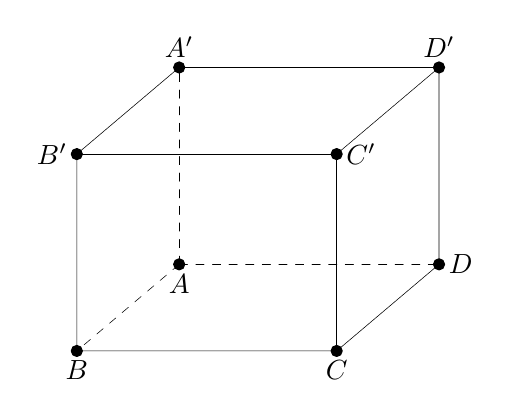
\begin{tikzpicture}[scale=1,>=stealth, font=\footnotesize, line join=round, line cap=round]
			\tkzDefPoints{0/0/A,-1.3/-1.1/B,2/-1.1/C}
			\coordinate (D) at ($(A)+(C)-(B)$);
			\coordinate (A') at ($(A)+(0,2.5)$);
			\tkzDefPointsBy[translation=from A to A'](B,C,D){B'}{C'}{D'}
			\tkzDrawPolygon(A',B',B,C,D,D')
			\tkzDrawSegments(B',C' C',D' C,C')
			\tkzDrawSegments[dashed](A,B A,D A,A')
			\tkzDrawPoints[fill=black,size=4](A,B,D,C,A',B',C',D')
			\tkzLabelPoints[above](A',D')
			\tkzLabelPoints[below](A,B,C)
			\tkzLabelPoints[left](B')
			\tkzLabelPoints[right](C',D)
		\end{tikzpicture}
		\vspace{10mm}
		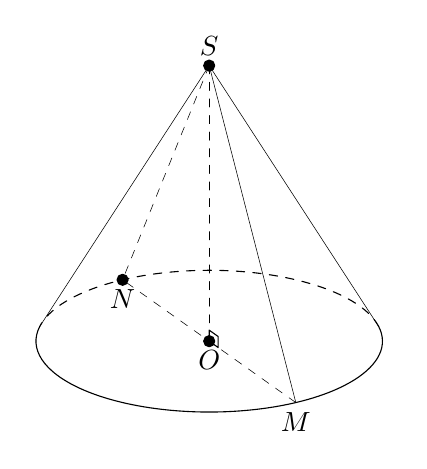
\begin{tikzpicture}[scale=1,>=stealth, font=\footnotesize, line join=round, line cap=round]
			\def \x{2.2} %bán kính trục lớn elip
			\def \y{0.9} %bán kính trục bé elip
			\def \h{3.5} %chiều cao hình nón
			\coordinate (O) at (0,0);
			\coordinate (S) at ($(O)+(0,\h)$);
			\coordinate (M) at (-60:\x cm and \y cm);
			\coordinate (N) at ($(O)!-1!(M)$);
			\coordinate (l) at (168:\x cm and \y cm);
			\coordinate (r) at (12:\x cm and \y cm);
			\draw[dashed] (r) arc (12:168:\x cm and \y cm);
			\draw (r) arc (12:-192:\x cm and \y cm);
			\tkzDrawSegments(S,l S,r S,M)
			\tkzDrawSegments[dashed](S,O M,N S,N)
			\tkzDrawPoints[fill=black,size=4](O,S,N)
			\tkzLabelPoints[above](S);
			\tkzLabelPoints[below](O,M,N);
			\tkzMarkRightAngles[size=0.14](S,O,M)
		\end{tikzpicture}
		
		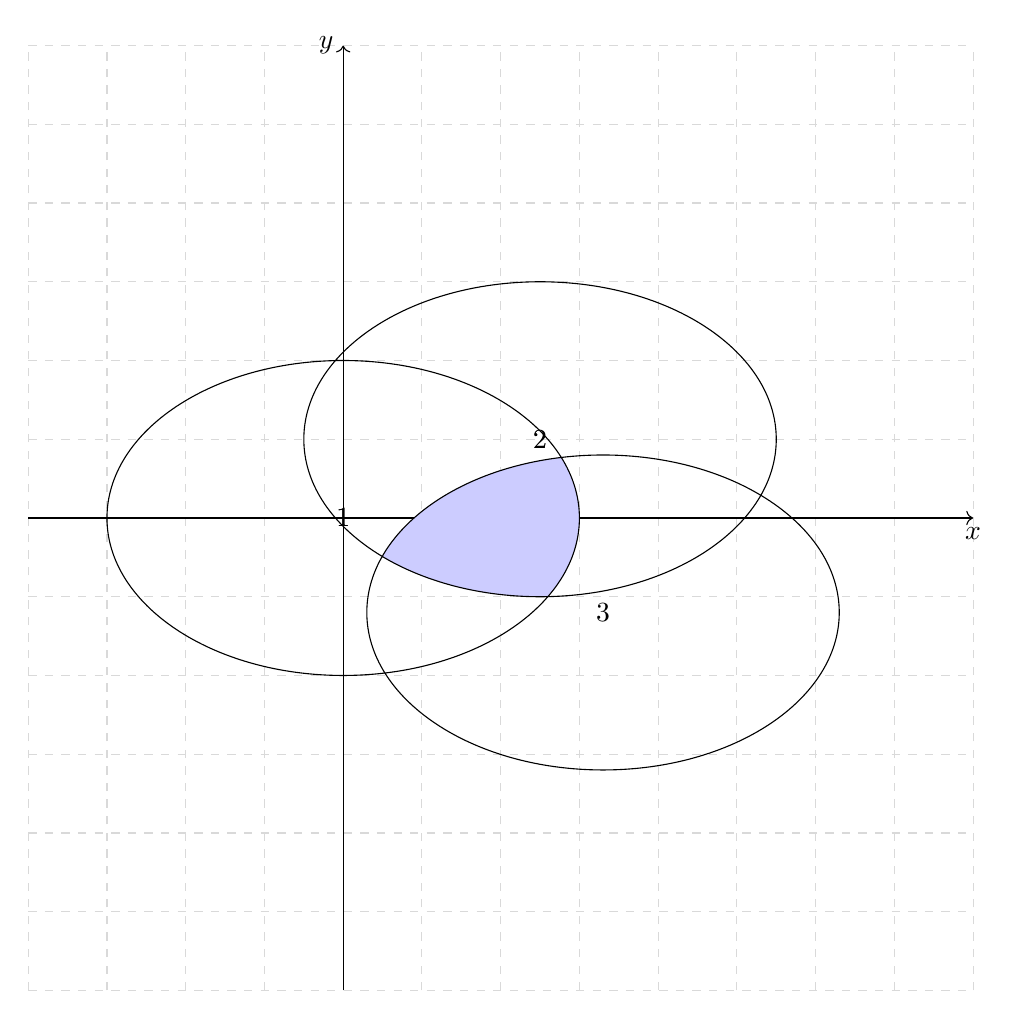
\begin{tikzpicture}[scale=1]
			\draw[color=gray!30,dashed] (-4,-6) grid (8,6);
			\draw[->] (-4,0)--(8,0) node [below]{$x$};
			\draw[->] (0,-6)--(0,6) node [left]{$y$};
			\clip (-4,-6) rectangle (8,6);
			%%%%%%%%
			\def\firstven{(0,0) ellipse (3cm and 2cm) node{1}}
			\def\secondven{(2.5,1) ellipse (3cm and 2cm) node{2}}
			\def\thirdven{(3.3,-1.2) ellipse (3cm and 2cm) node{3}}
			\begin{scope}
				\clip \firstven;
				\clip \secondven;
				\fill[blue!20] \thirdven;
			\end{scope}
			\draw \firstven \secondven \thirdven;
		\end{tikzpicture}

	%-------------------------
	\Closesolutionfile{ans}
	
\end{document}